\section{Thursday, September 22th}
\subsection{LCCDEs \& State-Space Resp. (continued)}
Draw a Delay-Adder-Gain (DAG) block diagram with minimum number of \textit{delay} blocks:
\begin{figure}[h]
    \centering
    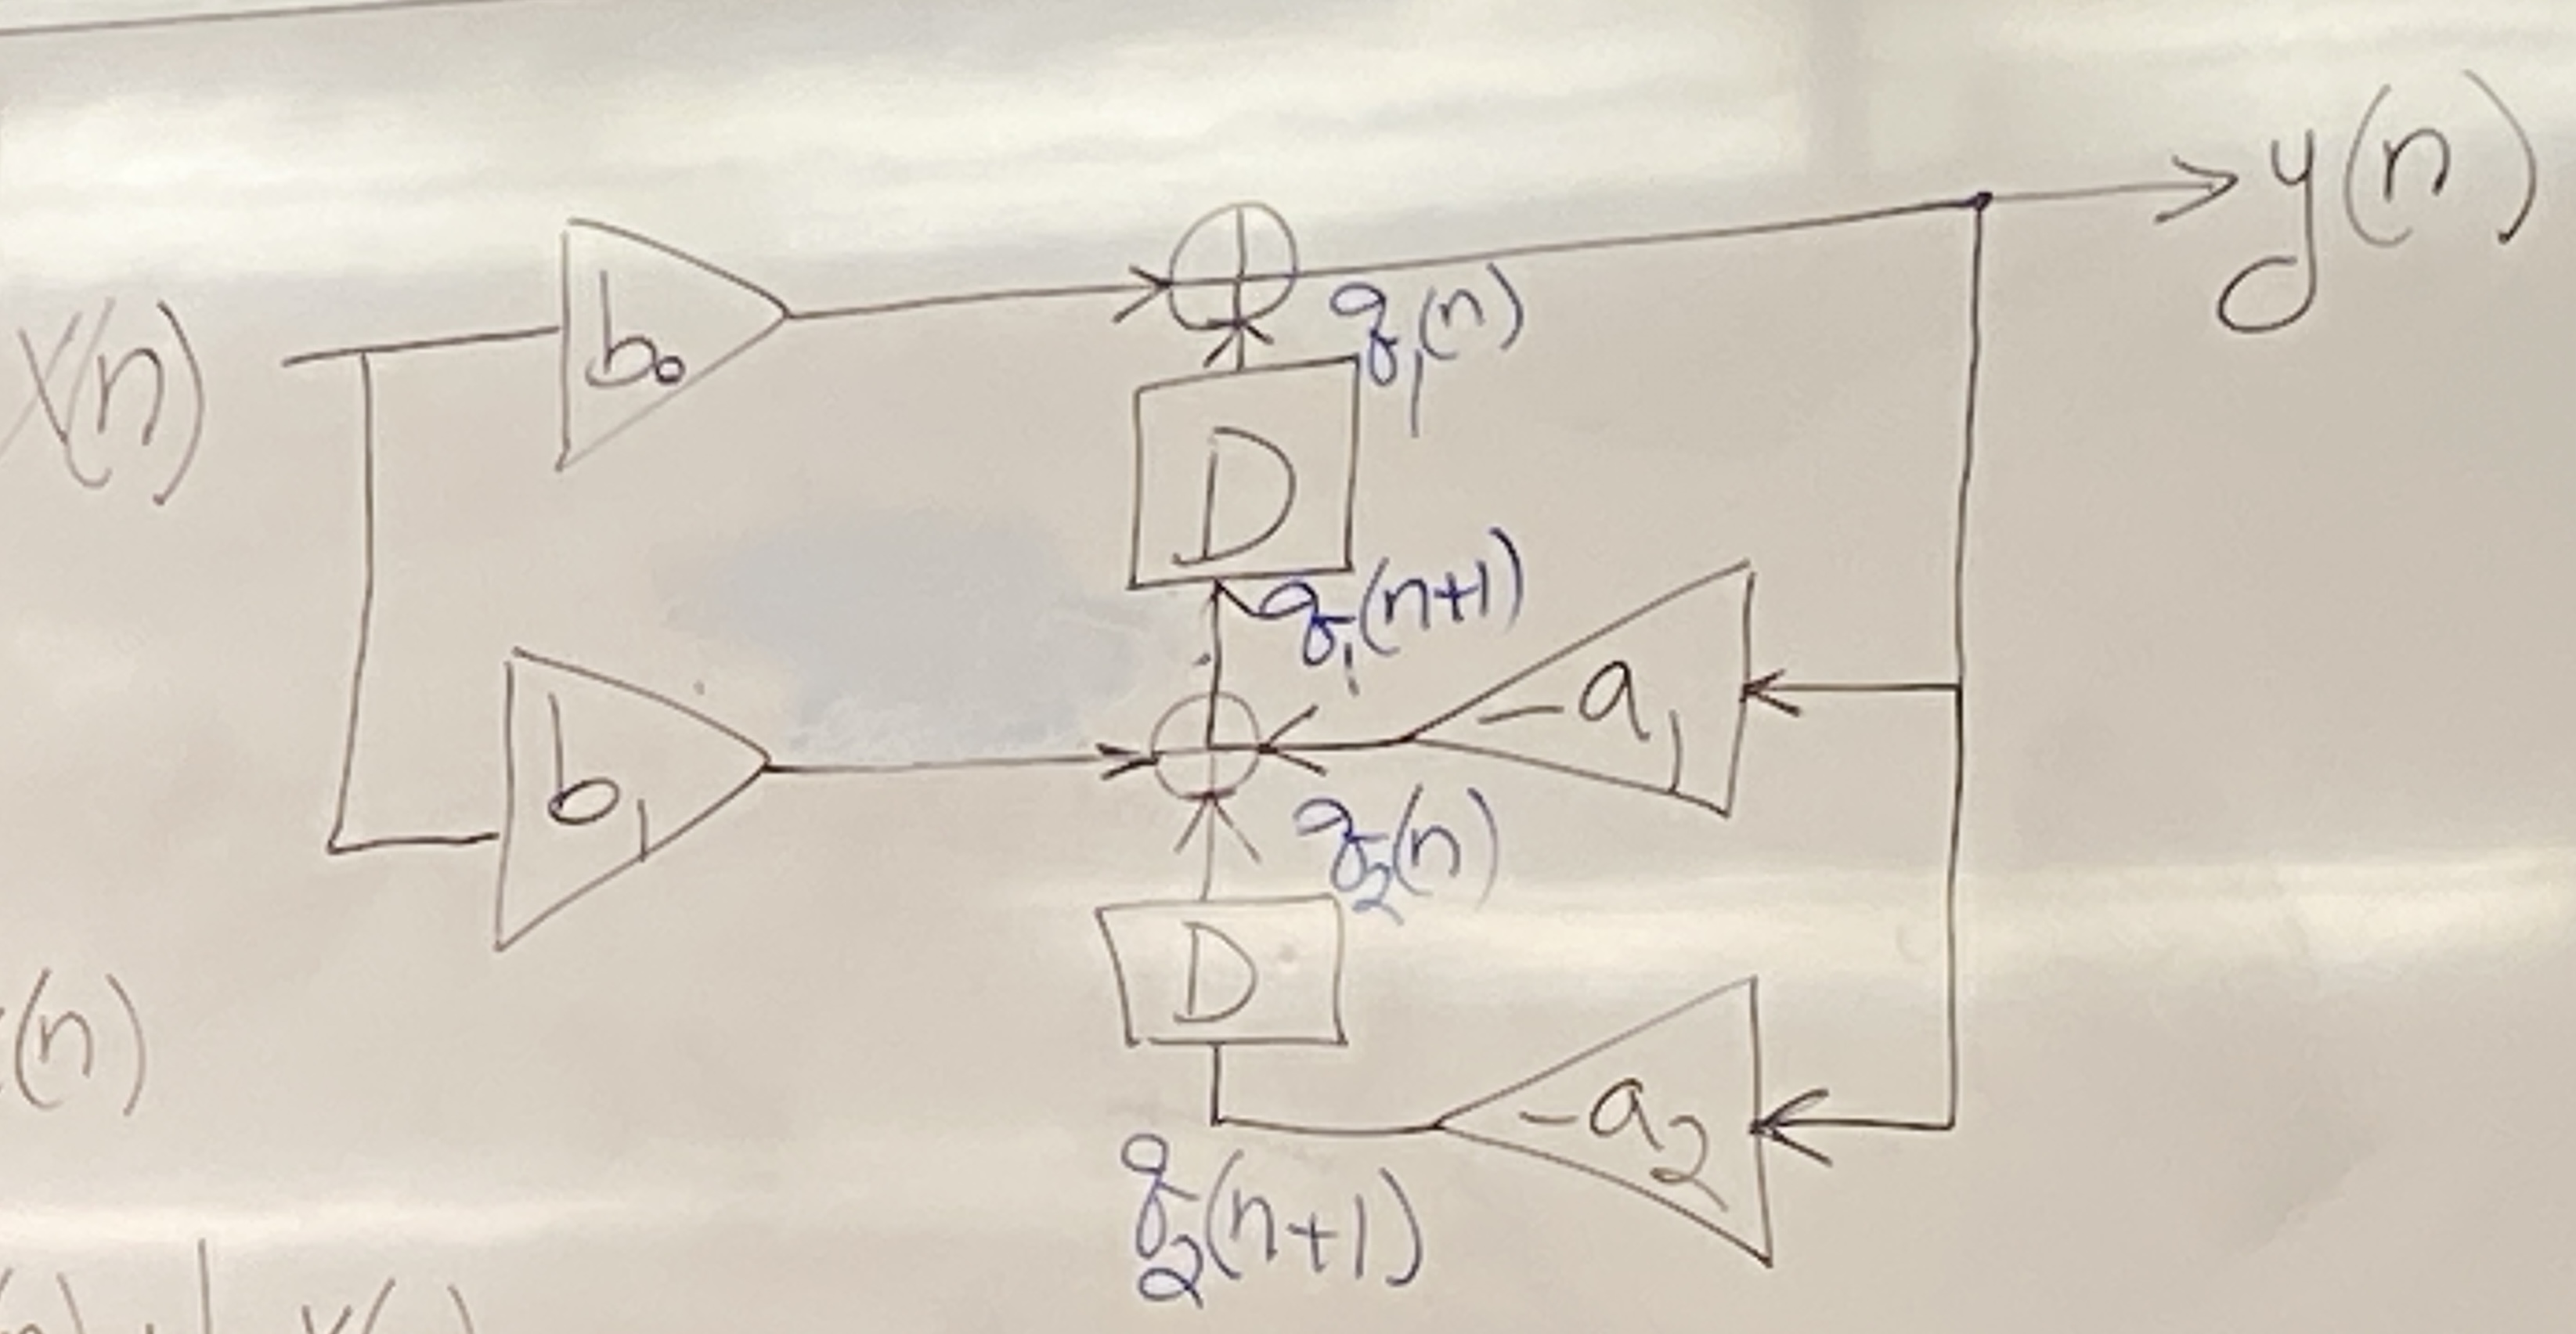
\includegraphics[scale=0.1]{lectures/img/Lec8_DAG.jpg}
    \label{fig:lec8_dag}
\end{figure}

\begin{align*}
    q(n+1) &= A q(n) + B x(n)
    \\
    y(n) &= C q(n) + D x(n)
    \\
    q(n) &= \begin{bmatrix}
        q_1(n) \\ q_2(n)
    \end{bmatrix}
\end{align*}

\begin{align*}
    y(n)
    &= q_1(n) + b_0 x(n)
    \\
    &= \underbrace{\begin{bmatrix}
        1 & 0
    \end{bmatrix}}_C \begin{bmatrix}
        q_1(n)\\
        q_2(n)
    \end{bmatrix}
    + \underbrace{b_0}_D x(n)
    \\
    q_1(n+1)
    &= -a_1 y(n) + q_2 + b_1 x(n)
    \\
    &= -a_1 \underbrace{\begin{bmatrix}
        q_1(n) + b_0 x(n)
    \end{bmatrix}}_{y(n)} + q_2(n) + b_1 x(n)
\end{align*}

\begin{align*}
    q_1(n+1) &= \begin{bmatrix}-a_1 & 1\end{bmatrix}
    \begin{bmatrix}
        q_1(n)\\
        q_2(n)
    \end{bmatrix}
    + \begin{bmatrix}
        b_1 - a_1 b_0
    \end{bmatrix} x(n)
    \\
    q_2(n+1) &= -a_2 y(n)  
    \\
    -a_2 \begin{bmatrix}
        .
    \end{bmatrix}
    \begin{bmatrix}
        q_1(n)\\
        q_2(n)
    \end{bmatrix}
    + (
        b_1 - a_1 b_0
    ) x(n)
\end{align*}

\subsection{Dirac Delta (CT Impulse)}
Recall that
\[
    \delta(n) = \begin{cases}
        1 & \quad n = 0
        \\
        0 & \quad \text{e/w}
    \end{cases}
\]
and that
\[
    \delta(t) = \begin{cases}
        \infty & \quad t = 0
        \\
        0 & \quad t\ne0
    \end{cases}
\]
but note that this is a useless description by itself -- but becomes useful when applied with Calculus.

This can be drawn out with an arrowhead instead of a lollipop.

Recall that Newton's Second Law states: $\vec F = \frac{\mathrm{d}\vec p}{\mathrm{d}t}$


Sampling Property:
\[
    x(t)\delta(t-t_0)
    =
    x(t_0)\delta(t-t_0)
\]

More generally:
\[
    \int_{-\infty}^\infty x(t)\delta(t-t_0) \mathrm d t = x(t_0)
\]
given that integral bounds $a \le t_0 \le b$ (otherwise you would just get 0).

Strength 1 = area 1.

\subsection{CT Convolution}
\[
    x(t) 
    = \int_{-\infty}^\infty x(\tau)\delta(t-\tau) \mathrm d\tau
\]

\subsection{CT Freq Resp}
If LTI:
\[
    x(t) 
    = \int_{-\infty}^\infty x(\tau)\delta(t-\tau) \mathrm d\tau
    \to
    \boxed{H}
    \to
    y(t) 
    = \int_{-\infty}^\infty h(\tau)\delta(t-\tau) \mathrm d\tau
\]
Let $\lambda = t - \tau 
\implies \tau=t-\lambda
\implies\d\lambda=-\d\tau$
